% !TeX program = PdfLaTeX
% !TeX root = ../../Elaborati_Aerodinamica_Bruno_Spoti.tex

\section{Campo di moto e aerodinamica non viscosa per fissati $\alpha$ e $M_{\infty}$}
Lo scopo di questo capitolo è quello di esporre i risultati ottenuti dalla completa risoluzione del campo di moto fissate le condizioni operative riportate in tabella~\ref{tabS3} e dall'analisi aerodinamica non viscosa dello stesso.

\begin{table} [!h]\centering \rowcolors{1}{}{grigio_chiaro}
	\begin{tabular}{c c c}
		\toprule
		\emph{\Minf } &  $\alpha$ & h \\ 
		\midrule
		3 & $0^{\circ}$ & 1000 m \\
		\bottomrule
	\end{tabular}
	\caption {\footnotesize Condizioni operative per l'analisi aerodinamica del profilo alare per il volo supersonico}
	\label{tabS3}
\end{table}

Utilizzando il modello dell'atmosfera \emph{standard} (\emph{ISA}), alla quota in esame l'aria si assume le caratteristiche di pressione densità e temperatura riportate in tabella~\vref{tabS4}

\begin{table} [!h]\centering \rowcolors{1}{}{grigio_chiaro}
	\begin{tabular}{c c c}
		\toprule
		\emph{$p_{\infty}$ } &  \emph{$T_{\infty}$ } & \emph{$\rho_{\infty}$ } \\ 
		\midrule
		26436.3 \si{\pascal} & $223.15 \si{\kelvin}$ & 0.413 \si{\kilo\gram\per\cubic\meter}\\
		\bottomrule
	\end{tabular}
	\caption {\footnotesize Condizioni asintotiche della corrente a quota 10000\si{\meter}}
	\label{tabS4}
\end{table} 

\subsection{Determinazione del campo di moto attorno al corpo e a valle}
Per ognuna delle regioni evidenziate in figura~\vref{figS4},
nota la geometria del corpo, è stata considerata un'onda d'urto o un'onda di espansione in funzione dell'angolo di deviazione locale della corrente e sono state calcolate tutte le caratteristiche a valle della stessa.

\begin{figure}[h!]
	\centering
	\begin{tikzpicture}
	\begin{axis}[ 
	axis lines=none,        %commentare per ritornare alla griglia
	xmin=-0.05, 
	xmax=1.40, 
	ymin=-0.15,
	ymax=0.15,
	xlabel=$ \frac {x}{c}$, 
	ylabel=$ \frac {z}{c}$,
	ylabel style={rotate=-90},
	ytick={-0.1,-0.05,0,0.05,0.1},
	yticklabels={$-0.1$,$-0.05$,$0$,$0.05$,$0.1$},
	width=13cm,
	height=2.69 cm,
	scale only axis,
	grid=major] 
	\addplot [black,solid, thick,mark options={solid}, mark size=2pt]
	file{images/fileDat/Parte_2-Profilo_supersonico/Geometria/Geometria.dat};
	\addplot [black,thin,solid,mark options={solid}]file{images/fileDat/Parte_2-Profilo_supersonico/Geometria/Mach_3_alpha_0/1_IntermediateWave1_2_alpha_0_Mach_3.dat};
	\addplot [black,thin,solid,mark options={solid}]file{images/fileDat/Parte_2-Profilo_supersonico/Geometria/Mach_3_alpha_0/1_IntermediateWave4_5_alpha_0_Mach_3.dat};
	\addplot [black,thin,solid,mark options={solid}]file{images/fileDat/Parte_2-Profilo_supersonico/Geometria/Mach_3_alpha_0/2_IntermediateWave4_5_alpha_0_Mach_3.dat};
	\addplot [black,thin,solid,mark options={solid}]file{images/fileDat/Parte_2-Profilo_supersonico/Geometria/Mach_3_alpha_0/3_IntermediateWave4_5_alpha_0_Mach_3.dat};
	\addplot [black,thin,solid,mark options={solid}]file{images/fileDat/Parte_2-Profilo_supersonico/Geometria/Mach_3_alpha_0/4_IntermediateWave4_5_alpha_0_Mach_3.dat};
	\addplot [black,thin,solid,mark options={solid}]file{images/fileDat/Parte_2-Profilo_supersonico/Geometria/Mach_3_alpha_0/FirstWave1_2_alpha_0_Mach_3.dat};
	\addplot [black,thin,solid,mark options={solid}]file{images/fileDat/Parte_2-Profilo_supersonico/Geometria/Mach_3_alpha_0/FirstWave4_5_alpha_0_Mach_3.dat};
	\addplot [black,thin,solid,mark options={solid}]file{images/fileDat/Parte_2-Profilo_supersonico/Geometria/Mach_3_alpha_0/LastWave1_2_alpha_0_Mach_3.dat};
	\addplot [black,thin,solid,mark options={solid}]file{images/fileDat/Parte_2-Profilo_supersonico/Geometria/Mach_3_alpha_0/LastWave1_2_alpha_0_Mach_3.dat};
	\addplot [black,very thick,solid,mark options={solid}]file{images/fileDat/Parte_2-Profilo_supersonico/Geometria/Mach_3_alpha_0/ShockWave0_1_alpha_0_Mach_3.dat};
	\addplot [black,very thick,solid,mark options={solid}]file{images/fileDat/Parte_2-Profilo_supersonico/Geometria/Mach_3_alpha_0/ShockWave0_4_alpha_0_Mach_3.dat};
	\addplot [black,very thick,solid,mark options={solid}]file{images/fileDat/Parte_2-Profilo_supersonico/Geometria/Mach_3_alpha_0/ShockWave2_3_alpha_0_Mach_3.dat};
	\addplot [black,very thick,solid,mark options={solid}]file{images/fileDat/Parte_2-Profilo_supersonico/Geometria/Mach_3_alpha_0/ShockWave5_6_alpha_0_Mach_3.dat};
	\addplot [black,very thick,solid,mark options={solid}]file{images/fileDat/Parte_2-Profilo_supersonico/Geometria/Mach_3_alpha_0/ShockWave5_6_alpha_0_Mach_3.dat};
	\addplot [black,dashed,mark options={solid}]file{images/fileDat/Parte_2-Profilo_supersonico/Geometria/Mach_3_alpha_0/SlipLine_alpha_0_Mach_3.dat};
	\node at (axis cs: 0.4, 0.07) { \scriptsize Regione 1};
	\node at (axis cs: 0.95, 0.07) { \scriptsize Regione 2};
	\node at (axis cs: 0.30, -0.1) { \scriptsize Regione 4};
	\node at (axis cs: 0.8, -0.1) { \scriptsize Regione 5};
	\node at (axis cs: 1.3, 0.04) { \scriptsize Regione 3};
	\node at (axis cs: 1.3, -0.05) { \scriptsize Regione 6};
	\end{axis}
	\end{tikzpicture}
	\caption{\footnotesize Notazione regioni in cui si divide il campo di moto}
	\label{figS4}
\end{figure}

Per il calcolo del campo di moto a valle del profilo, è stato implementato un procedimento iterativo, non essendo nota a priori la direzione della linea di slip, imponendo come criterio di convergenza che la differenza tra gli errori in due {/itshape step} successivi sia  minore di $10^-6$. Tale errore è valutato considerando che le pressioni nella regione 3 e nella regione 6 devono essere uguali. Il campo di moto ottenuto e riportato in figura~\vref{figS5}, dove l'inclinazione di tutte le onde è in scala reale, mentre i risultati per le diverse zone sono riportati in tabella~\vref{tabS5}

\begin{figure}[h!]
	\centering
	\begin{tikzpicture}[label distance= 1mm]
	\pgfplotsset{every y tick label/.append style={font=\footnotesize, xshift=0.5ex}}
	\pgfplotsset{every x tick label/.append style={font=\footnotesize}}
	\begin{axis}[ 
	%axis lines=none,        %commentare per ritornare alla griglia
	xmin=-0.1, 
	xmax=1.3, 
	ymin=-0.15,
	ymax=0.15,
	xlabel=$ \frac {x}{c}$, 
	ylabel=$ \frac {z}{c}$,
	y label style={at={(axis cs: -0.2,0 )},rotate=-90,anchor=center},
	ytick={-.1,-0.05,0,0.05,0.1},
	yticklabels={$-0.1$,$-0.05$,$0$,$0.05$,$0.1$},
	width=14cm,
	height=3 cm,
	scale only axis,
	grid=minor] 
	\addplot [black,solid, thick,mark options={solid}, mark size=2pt]
	file{images/fileDat/Parte_2-Profilo_supersonico/Geometria/Geometria.dat};
	\addplot [black,thin,solid,mark options={solid}]file{images/fileDat/Parte_2-Profilo_supersonico/Geometria/Mach_3_alpha_0/1_IntermediateWave1_2_alpha_0_Mach_3.dat};
	\addplot [black,thin,solid,mark options={solid}]file{images/fileDat/Parte_2-Profilo_supersonico/Geometria/Mach_3_alpha_0/1_IntermediateWave4_5_alpha_0_Mach_3.dat};
	\addplot [black,thin,solid,mark options={solid}]file{images/fileDat/Parte_2-Profilo_supersonico/Geometria/Mach_3_alpha_0/2_IntermediateWave4_5_alpha_0_Mach_3.dat};
	\addplot [black,thin,solid,mark options={solid}]file{images/fileDat/Parte_2-Profilo_supersonico/Geometria/Mach_3_alpha_0/3_IntermediateWave4_5_alpha_0_Mach_3.dat};
	\addplot [black,thin,solid,mark options={solid}]file{images/fileDat/Parte_2-Profilo_supersonico/Geometria/Mach_3_alpha_0/4_IntermediateWave4_5_alpha_0_Mach_3.dat};
	\addplot [black,thin,solid,mark options={solid}]file{images/fileDat/Parte_2-Profilo_supersonico/Geometria/Mach_3_alpha_0/FirstWave1_2_alpha_0_Mach_3.dat};
	\addplot [black,thin,solid,mark options={solid}]file{images/fileDat/Parte_2-Profilo_supersonico/Geometria/Mach_3_alpha_0/FirstWave4_5_alpha_0_Mach_3.dat};
	\addplot [black,thin,solid,mark options={solid}]file{images/fileDat/Parte_2-Profilo_supersonico/Geometria/Mach_3_alpha_0/LastWave1_2_alpha_0_Mach_3.dat};
	\addplot [black,thin,solid,mark options={solid}]file{images/fileDat/Parte_2-Profilo_supersonico/Geometria/Mach_3_alpha_0/LastWave1_2_alpha_0_Mach_3.dat};
	\addplot [black,very thick,solid,mark options={solid}]file{images/fileDat/Parte_2-Profilo_supersonico/Geometria/Mach_3_alpha_0/ShockWave0_1_alpha_0_Mach_3.dat};
	\addplot [black,very thick,solid,mark options={solid}]file{images/fileDat/Parte_2-Profilo_supersonico/Geometria/Mach_3_alpha_0/ShockWave0_4_alpha_0_Mach_3.dat};
	\addplot [black,very thick,solid,mark options={solid}]file{images/fileDat/Parte_2-Profilo_supersonico/Geometria/Mach_3_alpha_0/ShockWave2_3_alpha_0_Mach_3.dat};
	\addplot [black,very thick,solid,mark options={solid}]file{images/fileDat/Parte_2-Profilo_supersonico/Geometria/Mach_3_alpha_0/ShockWave5_6_alpha_0_Mach_3.dat};
	\addplot [black,very thick,solid,mark options={solid}]file{images/fileDat/Parte_2-Profilo_supersonico/Geometria/Mach_3_alpha_0/ShockWave5_6_alpha_0_Mach_3.dat};
	\addplot [black,dashed,mark options={solid}]file{images/fileDat/Parte_2-Profilo_supersonico/Geometria/Mach_3_alpha_0/SlipLine_alpha_0_Mach_3.dat};
	\addplot [black,ultra thin,mark options={solid}]file{images/fileDat/Parte_2-Profilo_supersonico/Geometria/Mach_3_alpha_0/flowLine_k_0.1.dat};
	\addplot [black,ultra thin,mark options={solid}]file{images/fileDat/Parte_2-Profilo_supersonico/Geometria/Mach_3_alpha_0/flowLine_k_-0.1.dat};
	\addplot [black,ultra thin,mark options={solid}]file{images/fileDat/Parte_2-Profilo_supersonico/Geometria/Mach_3_alpha_0/flowLine_k_0.02.dat};
	\addplot [black,ultra thin,mark options={solid}]file{images/fileDat/Parte_2-Profilo_supersonico/Geometria/Mach_3_alpha_0/flowLine_k_-0.02.dat};
	\addplot [black,ultra thin,mark options={solid}]file{images/fileDat/Parte_2-Profilo_supersonico/Geometria/Mach_3_alpha_0/flowLine_k_0.02.dat};
	\addplot [black,ultra thin,mark options={solid}]file{images/fileDat/Parte_2-Profilo_supersonico/Geometria/Mach_3_alpha_0/flowLine_k_-0.2.dat};
	\addplot [black,ultra thin,mark options={solid}]file{images/fileDat/Parte_2-Profilo_supersonico/Geometria/Mach_3_alpha_0/flowLine_k_0.2.dat};
	\addplot [black,ultra thin,mark options={solid}]file{images/fileDat/Parte_2-Profilo_supersonico/Geometria/Mach_3_alpha_0/flowLine_k_-0.3.dat};
	\addplot [black,ultra thin,mark options={solid}]file{images/fileDat/Parte_2-Profilo_supersonico/Geometria/Mach_3_alpha_0/flowLine_k_0.3.dat};
	\addplot [black,ultra thin,mark options={solid}]file{images/fileDat/Parte_2-Profilo_supersonico/Geometria/Mach_3_alpha_0/flowLine_k_-0.04.dat};
	\addplot [black,ultra thin,mark options={solid}]file{images/fileDat/Parte_2-Profilo_supersonico/Geometria/Mach_3_alpha_0/flowLine_k_0.04.dat};
	\addplot [black,ultra thin,mark options={solid}]file{images/fileDat/Parte_2-Profilo_supersonico/Geometria/Mach_3_alpha_0/flowLine_k_-0.06.dat};
	\addplot [black,ultra thin,mark options={solid}]file{images/fileDat/Parte_2-Profilo_supersonico/Geometria/Mach_3_alpha_0/flowLine_k_0.06.dat};
	\addplot [black,ultra thin,mark options={solid}]file{images/fileDat/Parte_2-Profilo_supersonico/Geometria/Mach_3_alpha_0/flowLine_k_-0.08.dat};
	\addplot [black,ultra thin,mark options={solid}]file{images/fileDat/Parte_2-Profilo_supersonico/Geometria/Mach_3_alpha_0/flowLine_k_0.08.dat};
	\addplot [black,ultra thin,mark options={solid}]file{images/fileDat/Parte_2-Profilo_supersonico/Geometria/Mach_3_alpha_0/flowLine_k_-0.12.dat};
	\addplot [black,ultra thin,mark options={solid}]file{images/fileDat/Parte_2-Profilo_supersonico/Geometria/Mach_3_alpha_0/flowLine_k_0.12.dat};
	\addplot [black,ultra thin,mark options={solid}]file{images/fileDat/Parte_2-Profilo_supersonico/Geometria/Mach_3_alpha_0/flowLine_k_-0.14.dat};
	\addplot [black,ultra thin,mark options={solid}]file{images/fileDat/Parte_2-Profilo_supersonico/Geometria/Mach_3_alpha_0/flowLine_k_0.14.dat};
	\addplot [black,ultra thin,mark options={solid}]file{images/fileDat/Parte_2-Profilo_supersonico/Geometria/Mach_3_alpha_0/flowLine_k_-0.16.dat};
	\addplot [black,ultra thin,mark options={solid}]file{images/fileDat/Parte_2-Profilo_supersonico/Geometria/Mach_3_alpha_0/flowLine_k_0.16.dat};
	\draw[-latex] (axis cs:-0.11, 0) -- (axis cs:-0.02, 0);
	
	\node at (axis cs: 0.35, 0.07) { \scriptsize  1};
	\node at (axis cs: 0.95, 0.07) { \scriptsize  2};
	\node at (axis cs: 0.28, -0.08) { \scriptsize  4};
	\node at (axis cs: 0.75, -0.075) { \scriptsize  5};
	\node at (axis cs: 1.25, 0.036) { \scriptsize  3};
	\node at (axis cs: 1.25, -0.037) { \scriptsize  6};
	\end{axis}
	\end{tikzpicture}
	\caption{\footnotesize Schematizzazione campo di moto per $\alpha=0^\circ$ e $\Minf=3$ con inclinazione onde in scala reale}
	\label{figS5}
\end{figure}

\begin{table} [!h]\centering \rowcolors{1}{}{grigio_chiaro}
	\begin{tabular}{l  c  c c c c c}
		\toprule
		& \emph{Regione 1}& \emph{Regione 2}& \emph{Regione 3}& \emph{Regione 4}& \emph{Regione 5}& \emph{Regione 6}   \\ 
		\midrule
		$M$	&	2.90	&	3.15	&	3.00	&	2.52	&	3.26	&	2.97	\\
		$p/p_{\infty}$ &   1.158	&	0.7965	&	1.001	&	2.018	&	0.6559	&	1.001	\\
		$p \ [\si{Pa}]$	&	30601.6	&	21057.8	&	26456.8	&	53338.4	&	17338.7	&	26456.9	\\
		$T/T_{\infty}$ &  1.043	&	0.9372	&	1.001	&	1.234	&	0.8953	&	1.012	\\
		$T \ [\si{K}]$	&	232.7	&	209.1	&	223.3	&	275.4	&	199.8	&	225.9	\\
		$\rho/\rho_{\infty}$ & 1.110	&	0.8500	&	1.000	&	1.635	&	0.7325	&	0.988	\\
		$\rho \ [\si{kg/m^3}]$	&	0.458	&	0.351	&	0.413	&	0.675	&	0.302	&	0.408	\\
		%$\mu$ &  1.37 & 1.37 & 1.37 & 1.37 & 1.37 & 1.37     \\
		%$\epsilon$ &  1.37 & 1.37 & 1.37 & 1.37 & 1.37 & 1.37   \\
		%$\delta$ &  1.37 & 1.37 & 1.37 & 1.37 & 1.37 & 1.37   \\
		\bottomrule
	\end{tabular}
	\caption {\footnotesize Grandezze descrittive del campo di moto per $\alpha=0^\circ$ e $\Minf=3$}
	\label{tabS5}
\end{table}

\begin{figure}[h!]
	\centering
	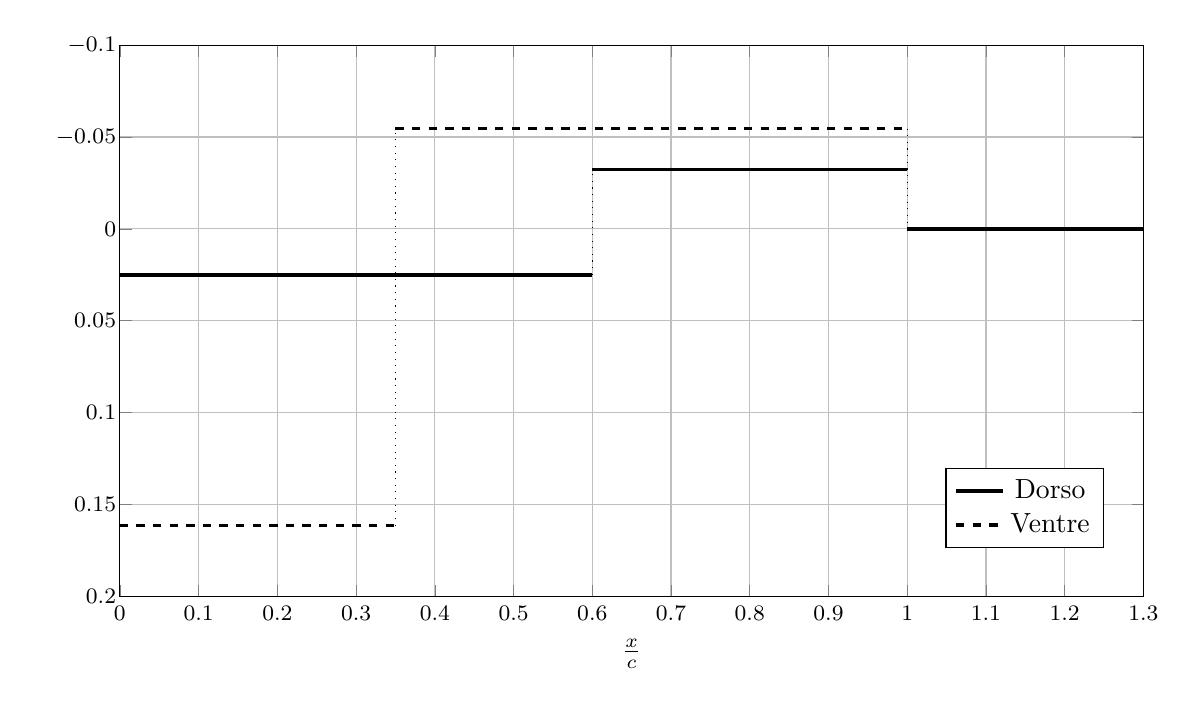
\begin{tikzpicture}
	\begin{axis}[ 	legend style={at={(axis cs: 1.25,0.13)}},
	xmin=0, 
	xmax=1.3, 
	ymin=-0.1, ymax=0.2,
	y dir=reverse,
    xlabel=$\frac{x}{c}$, 
	ylabel=\Cp,
	ylabel style={rotate=-90},
	ytick={-0.1,-0.05,0,0.05,0.1,0.15,0.2},
	yticklabels={$-0.1$,$-0.05$,$0$,$0.05$,$0.1$,$0.15$,$0.2$},
	width=13cm,
	height=7cm,
	scale only axis,
	grid=major] 
	
\addplot[line width=1.2pt] coordinates {( 0  ,  0.025009411302387) (0.60 ,  0.025009411302387)};
\addplot[dashed,line width=1.2pt] coordinates { (0  ,   0.161527192237048) (0.35  ,   0.161527192237048)};
\draw [line width=1.2pt]  (axis cs:0.6 , -0.032294126498668)-- (axis cs:1.0 , -0.032294126498668);
\draw [line width=1.2pt]  (axis cs:1.0 ,  0.000123039289931) -- (axis cs: 1.3 ,  0.000123039289931);


\draw [dashed,line width=1.2pt] (axis cs:0.35  ,  -0.054624164631687)-- (axis cs:1.00  ,  -0.054624164631687);
\draw  [dashed,line width=1.2pt] (axis cs:1.00  ,   0.000123531576380)-- (axis cs:1.30  ,   0.000123531576380);

\draw [dotted] (axis cs:0.60 ,  0.025009411302387) -- (axis cs:0.6 , -0.032294126498668);
%\draw[dotted] (axis cs:1.0 , -0.032294126498668) -- (axis cs:1.0 ,  0.000123039289931);

\draw [dotted] (axis cs:0.35  ,   0.161527192237048) -- (axis cs:0.35  ,  -0.054624164631687);
\draw[dotted] (axis cs:1.00  ,  -0.054624164631687) -- (axis cs:1.00  ,   0.000123531576380);

\legend{Dorso,Ventre}
	\end{axis}
	\end{tikzpicture}
	\caption{\footnotesize Coefficiente di pressione lungo il profilo con \Minf=3 e $\alpha=0^\circ$. MATLAB R2016b}
	\label{figS5bis}
\end{figure}



\subsection{Calcolo delle caratteristiche aerodinamiche}

Note le distribuzioni delle pressioni sulle quattro facce del quadrilatero, e la geometria dello stesso, è stato possibile ottenere le forze normali e tangenziali, i relativi coefficienti, le forze di portanza e resistenza, i coefficienti aerodinamici e il coefficiente di momento rispetto al bordo d'attacco, i cui risultati sono riportati in tabella~\vref{tabS6}
%Per il calcolo del centro di pressione è stato imposto nullo il momento aerodinamico e trascurata la componente lungo y dello stesso, ipotesi ammissibile per la sottigliezza del profilo.
L'ascissa del centro di pressione è stato riportato in figura~\vref{figS6} al variare dell'angolo d'attacco, fissato il numero di Mach, per apprezzarne il suo movimento.

\begin{table} [!h]\centering \rowcolors{1}{}{grigio_chiaro}
	\begin{tabular}{c c}
		\toprule
		\multicolumn{2}{c}{{\emph Grandezze aerodinamiche}}  \\ 
		\midrule
		$l$ &   3154.57 \si{N/m}\\ 
		$d$ &   2350.86 \si{N/m}\\ 
		$C_l$ &  0.0189\\ 
		$C_d$ &   141.15 (Drag Counts)\\ 
		$m_{le}$ &   1309.53 \si{(N/m).m}\\ 
		$C_{m_{le}}$ & 0.0079\\ 
		$C_{m_{ac}}$ &  0.0166 \\ 
		$\overline{x}_{cp}$ &   -0.415 \\
		\bottomrule
	\end{tabular}
	\caption {\footnotesize Grandezze descrittive del campo di moto per $\alpha=0^\circ$ e $\Minf=3$}
	\label{tabS6}
\end{table}


\begin{figure} [h!]
	\centering
	\begin{tikzpicture} 
	\begin{axis} [ 
	ylabel style={rotate=-90}, xmin=-8, 
	xmax=8, 
	ymin=-1,
	ymax=1.8,
	xlabel=$ {\alpha}$, 
	ylabel=$\frac{x_{cp}}{c}$,
	width=9cm,
	height=7 cm,
	scale only axis,
	grid=major] 
	\addplot [black,smooth]
	file{images/fileDat/Parte_2-Profilo_supersonico/CentroPressione/xcp_vs_alpha_Mach_3_ramo_negativo.dat};
	\addplot [black,smooth]
	file{images/fileDat/Parte_2-Profilo_supersonico/CentroPressione/xcp_vs_alpha_Mach_3_ramo_positivo.dat};
	\end{axis}
	\end{tikzpicture}
	\caption{\footnotesize Ascissa del centro di pressione al variare di ${\alpha}$. MATLAB R2016b}
	\label{figS6}
\end{figure}